\section{Planned Improvements}
\label{sec:production}

In parallel with its software development, the collaboration operates
a federated cloud infrastructure with sites in Orsay, France and
Athens, Greece\@.  These sites share a common user authentication
framework and Marketplace allowing users to allocate resources and to
use appliances on either site.  The collaboration uses this production
cloud to validate its software in real world conditions.

\begin{table}
\caption{Marketplace Statistics}
\label{table:statistics}
\begin{center}
\begin{tabular}{lr}
\hline
\hline
endorsers & 44 \\
current appliances & 105 \\
deprecated appliances & 170 \\
expired appliances & 832 \\
\hline
\hline
\end{tabular}
\end{center}
\end{table}

\begin{figure}
\begin{center}
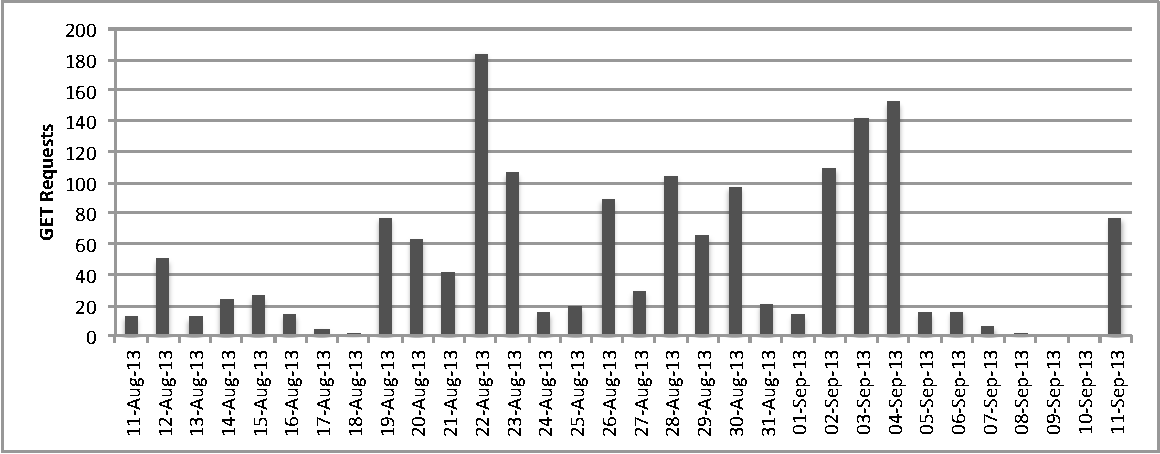
\includegraphics[width=\columnwidth]{getrequests.pdf}
\end{center}
\caption{Marketplace GET Requests}
\label{fig:requests}
\end{figure}

As a core service, the Marketplace is heavily used by both members of
the collaboration and users of the federated cloud.  Some statistics
on its use can be found in Table~\ref{table:statistics}.  
Figure~\ref{fig:requests} shows the number of daily requests for 
metadata over a month long period. Overall the service has performed well, 
with minor problems being addressed as the software evolves over time.  
Some outstanding issues and potential solutions are described below.

\subsection{Availability}

Having a central Marketplace instance allows users to easily find all
of the appliances from a single location.  Similarly, it allows image
creators to upload the metadata just once.  However, the Marketplace
is consulted every time a new machine instance is launched to check if
an appliance has been deprecated.  Consequently if the Marketplace is
not available, new instances cannot be created on any cloud relying on
the Marketplace\@.  Future iterations of the Marketplace must provide
redundancy and high-availability of the Marketplace service. 

To provide for this, a replication scheme will be implemented that
allows for multiple Marketplace instances to be deployed, each
maintaining a local copy of the metadata entries. As all the
information required to rebuild the metadata index stored in Sesame is
the set of raw metadata files, it is only these that need be
replicated.  A potential solution would be to use a Git repository as
the core `database' for the metadata entries, with each Marketplace
updating its index periodically from a local clone of the global
repository.

\subsection{Data Protection}

By design the appliance metadata is considered public.  In reality,
however, both users and administrators would like to restrict the
visibility of the appliance metadata for certain appliances.  Many
cloud administrators would like to run a ``private'' Marketplace to
limit the visibility of certain appliances while still taking
advantage of the central, public Marketplace instance.

There must be a mechanism for federating Marketplace instances in the
future and the move to using Git for metadata file management may also
facilitate the federation of different Marketplace instances.

\subsection{Appliance Quality}

Although the metadata contains a significant amount of information
about an appliance, it does not contain information about how well the
appliance functions for users.  A common request has been to add
social features to the Marketplace to allow users of an appliance to
leave comments and to signal problems with the appliance itself.  A
possible approach to add these features without overly complicating
the Marketplace implementation would be to make use of an external
service such as Disqus~\cite{disqus}.

\subsection{Appliance Evolution}

Appliances naturally evolve as operating system updates are applied
and new services are added.  However each time an appliance is
updated, the SHA-1 hash and the corresponding appliance identifier
change.  This makes it difficult for users to track the evolution of
an appliance and impossible to use a stable identifier for, for
example, the latest version of the CentOS appliance.

Recently a `tag' feature has been added to the Marketplace\@.  This
allows an endorser to provide a simple label for a series of
appliances, where the tag (namespaced by the endorser's email) will
always resolve to the latest appliance identifier.  By using the tag,
users can always use the latest version of an appliance without having
to find the associated identifier manually.

A complementary and more rigorous solution would be to make use of the
Dublin Core terms \emph{replaces} and \emph{isReplacedBy}. This would
provide a link in each metadata entry to the previous and next entries
in the evolution of the appliance.  The StratusLab tools must be
updated to simplify the use of these terms to ensure that they are
widely used.
